\documentclass[reprint,english,notitlepage]{revtex4-2}  % defines the basic parameters of the document

% if you want a single-column, remove reprint

% allows special characters (including æøå)
\usepackage[utf8]{inputenc}
\usepackage[english]{babel}

%% note that you may need to download some of these packages manually, it depends on your setup.
%% I recommend downloading TeXMaker, because it includes a large library of the most common packages.

\usepackage{physics,amssymb}  % mathematical symbols (physics imports amsmath)
\usepackage{graphicx}         % include graphics such as plots
\graphicspath{ {./Figures/} }
\usepackage{xcolor}           % set colors
\usepackage{hyperref}         % automagic cross-referencing (this is GODLIKE)
\usepackage{tikz}             % draw figures manually
\usepackage{listings}         % display code
\usepackage{subfigure}        % imports a lot of cool and useful figure commands
\usepackage[section]{placeins}

% defines the color of hyperref objects
% Blending two colors:  blue!80!black  =  80% blue and 20% black
\hypersetup{ % this is just my personal choice, feel free to change things
    colorlinks,
    linkcolor={red!50!black},
    citecolor={blue!50!black},
    urlcolor={blue!80!black}}

%% Defines the style of the programming listing
%% This is actually my personal template, go ahead and change stuff if you want
\lstset{ %
	inputpath=,
	backgroundcolor=\color{white!88!black},
	basicstyle={\ttfamily\scriptsize},
	commentstyle=\color{magenta},
	language=Python,
	morekeywords={True,False},
	tabsize=4,
	stringstyle=\color{green!55!black},
	frame=single,
	keywordstyle=\color{blue},
	showstringspaces=false,
	columns=fullflexible,
	keepspaces=true}


%% USEFUL LINKS:
%%
%%   UiO LaTeX guides:        https://www.mn.uio.no/ifi/tjenester/it/hjelp/latex/ 
%%   mathematics:             https://en.wikibooks.org/wiki/LaTeX/Mathematics

%%   PHYSICS !                https://mirror.hmc.edu/ctan/macros/latex/contrib/physics/physics.pdf

%%   the basics of Tikz:       https://en.wikibooks.org/wiki/LaTeX/PGF/TikZ
%%   all the colors!:          https://en.wikibooks.org/wiki/LaTeX/Colors
%%   how to draw tables:       https://en.wikibooks.org/wiki/LaTeX/Tables
%%   code listing styles:      https://en.wikibooks.org/wiki/LaTeX/Source_Code_Listings
%%   \includegraphics          https://en.wikibooks.org/wiki/LaTeX/Importing_Graphics
%%   learn more about figures  https://en.wikibooks.org/wiki/LaTeX/Floats,_Figures_and_Captions
%%   automagic bibliography:   https://en.wikibooks.org/wiki/LaTeX/Bibliography_Management  (this one is kinda difficult the first time)
%%   REVTeX Guide:             http://www.physics.csbsju.edu/370/papers/Journal_Style_Manuals/auguide4-1.pdf
%%
%%   (this document is of class "revtex4-1", the REVTeX Guide explains how the class works)


%% CREATING THE .pdf FILE USING LINUX IN THE TERMINAL
%% 
%% [terminal]$ pdflatex template.tex
%%
%% Run the command twice, always.
%% If you want to use \footnote, you need to run these commands (IN THIS SPECIFIC ORDER)
%% 
%% [terminal]$ pdflatex template.tex
%% [terminal]$ bibtex template
%% [terminal]$ pdflatex template.tex
%% [terminal]$ pdflatex template.tex
%%
%% Don't ask me why, I don't know.

\begin{document}
\title{FYS-STK3155 - Project 3}   % self-explanatory
\author{Dag Arne Lydvo}               % self-explanatory
\date{\today}                             % self-explanatory
\noaffiliation                            % ignore this
\begin{abstract}                          % marks the beginning of the abstract
 In this project I will train multiple machine learning models for the classification of whether a terror incident extends beyond 24 hours in length. The dataset is extracted from the Global Terrorism database. I will train both dense neural networks and support vector machine classification models. The models will show fairly good performance and little variance in performance between models, but some difference between activation functions used in the neural networks.  
\end{abstract}                            % marks the end of the abstract
\maketitle                                % creates the title, author, date & abstract


% the fundamental components of scientific reports:
\section{Introduction}
This project will analyse the Global Terrorism database of over 180 000 incidents of terror since 1970, with over 130 features. I will seek to select and narrow down the number of features for training the model. The target variable will be the "extended" features that describes whether a terror incident extends over 24 hours or not. It thus becomes a binary classification problem. I will replace values, create new feature and remove rows to try and solve the problem of missing values and thereby reducing the data set significantly. 

I will then seek to train models for the classification of a extended incident or not by first using feed forward dense neural networks of different architecture. I will then train support vector machine models to do the same classification and do a comparison of the the two different methods. 

\section{Method}
\subsection{Neural Network}
First model for classification is a ordinary feed forward neural network as described in project 2. 

\subsection{Suport Vector Machines}
I will in this project be using support vector machines for classification. A linear SVM seeks to divide samples by a line (if two dimension, called hyperplane), but with a given margin on each side with equal distance from the hyperplane.  
\begin{figure}[!htb]
	\centering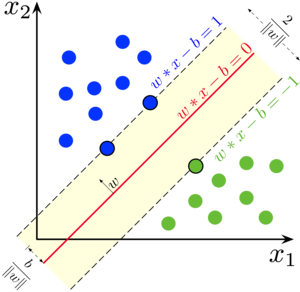
\includegraphics[trim=0 0 0 0, scale=2]{300px-SVM_margin}
	\caption{A hyperplance with margins [2]}\label{figure}
\end{figure}

\subsection{Accuracy score}
For classification an accuracy score is used 
\[ Accuracy = \frac{\sum_{i=1}^{n}I(t_i=y_i)}{n}\]
The accuracy scores measure the number of successful classifications over the number of data points being classified. The function I here produces 1 if classification is successful otherwise 0. 

\subsection{Datasets}
\subsubsection{Global Terrorism Database}
The dataset used for this project is the Global Terrorism database [1] found on Kaggle.com. The dataset contains 181 691 incidents of terrorism described by 135 features.

The dataset has been trimmed down first by a selection process where I collected the features I found to be of most interest. After this process the dataset was narrowed down to about 33 features and 1 target variable. See the jupyter notebook and the documentation for the dataset, Codebook.pdf for more in depth information on the selected features. 

\subsubsection{Feature extraction and missing values}
Several features had missing values and this where resolved by various methods.   

There was one new feature create, the multitypeattack. This feature is valued 1 if the incident had more than one class of attack type given by the features [attacktype1, attacktype2, attacktype3] otherwise 0. The features [attacktype2, attacktype3] where then removed.  

Many of the features where not systematically collected before 1997. And I decided to limit the dataset to incidents after 1997 (from 1/1/1998). This reduced the dataset to about 114 184 datapoints, but also helped solve for missing values. The features [nhostkid, alternative, propvalue, weapsubtype1, targsubtype1] had a lot of missing values and I decided to drop these features altogether. 

Further the features [nperps, nwound, nkill, natlty1] had missing values that where filled with -99 as this was a value used to describe unknown or unclassified instances of features in the database and I decided to fill missing values with this value. 

The remaining missing values where solved by droping rows containing missing values and after this I ended up with a dataset of 112 874 instances and 27 features and 1 target variable. The target variable is the "extended" feature of the dataset which describes whether or not an incident extended more than 24 hours, thus valued 1 if extended more than 24 hours else 0.   



\newpage


\section{Results}
\subsection{Neural networks}
First four experiments will be running neural networks. The first two will have a simple structure with two hidden layers of 100 and 50 neurons and with batch size of 10000 and running 10 epochs.
All networks will be using SGD optimizer and the sparse categorical crossentropy loss function. 
\newline

First neural network model using two hidden layers with 100 and 50 neurons and using the RELU activation functions for the hidden layers.
\begin{figure}[!htb]
	\centering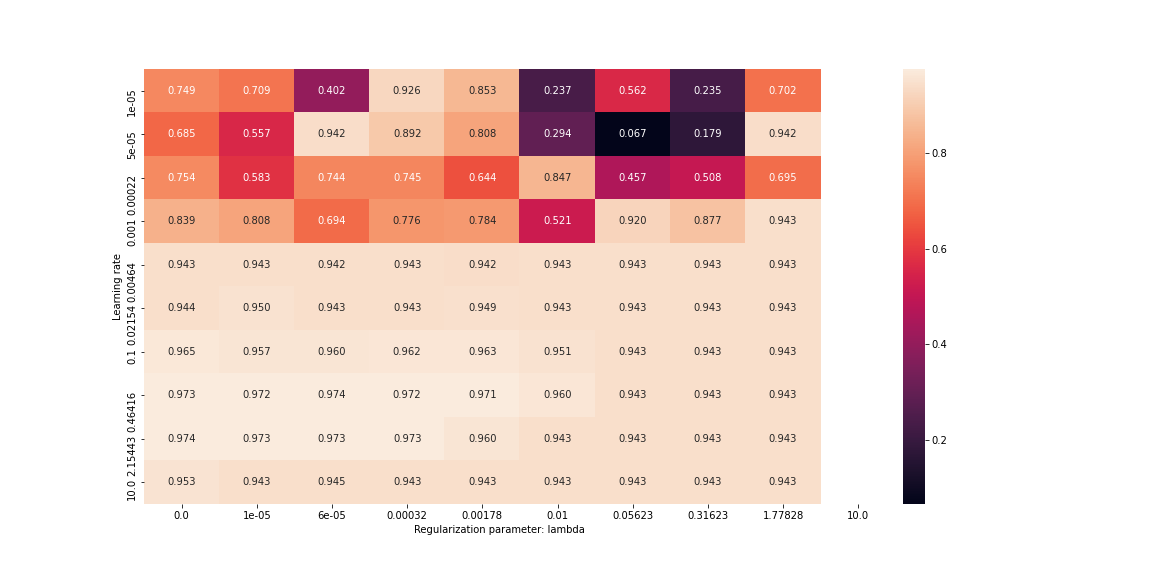
\includegraphics[trim=140 20 100 0, scale=0.3]{NNClass2}
	\caption{Accuracy score for first neural network model ploted over learning rate and regularization parameter.  }\label{figure}
\end{figure}
\newline

The second neural network model using two hidden layers with 100 and 50 neurons, but now using the ELU activation function for the hidden layers. 
\begin{figure}[!htb]
	\centering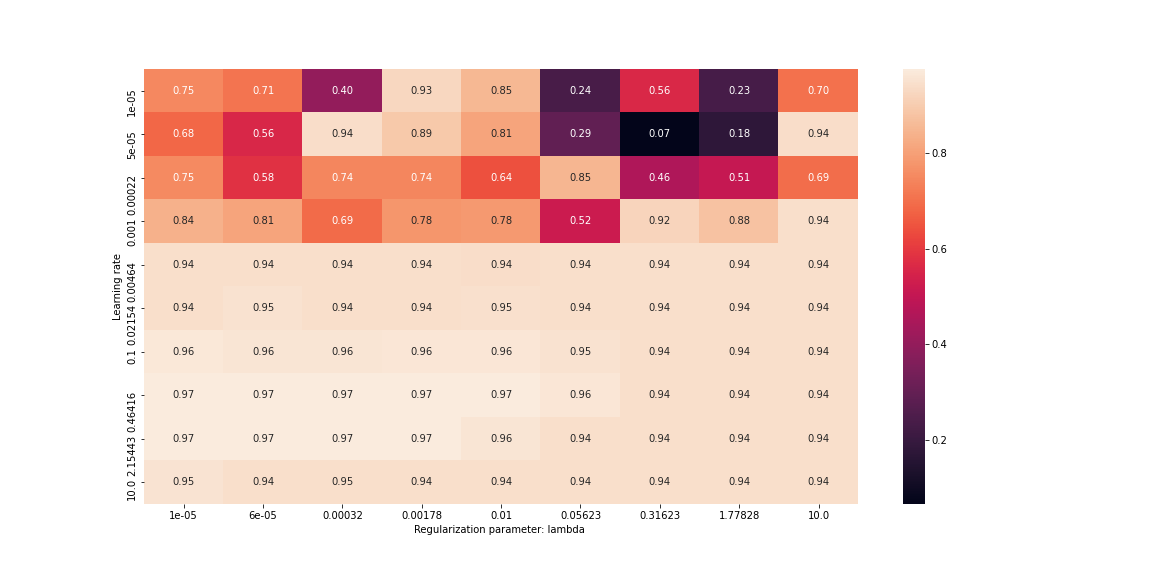
\includegraphics[trim=140 20 100 0, scale=0.3]{NNClass3}
	\caption{Accuracy score for second neural network model ploted over learning rate and regularization parameter.  }\label{figure}
\end{figure}

The third neural network model now has three hidden layers with 250,100 and 50 neurons and the batch size is half the size of the previous models with 5000 and the epochs have doubled to 20. Third model is using the RELU activation function. 
\begin{figure}[!htb]
	\centering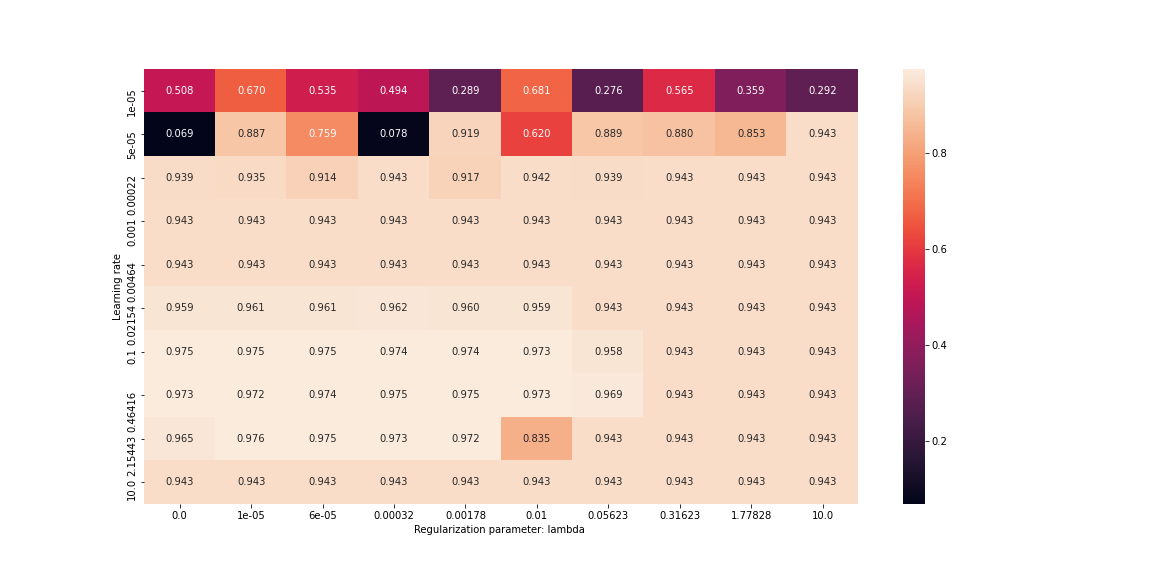
\includegraphics[trim=140 20 100 0, scale=0.3]{NNClass4}
	\caption{Accuracy score for third neural network model ploted over learning rate and regularization parameter.  }\label{figure}
\end{figure}

The fourth neural network model is equal to the third, but now using the ELU activation function.  
\begin{figure}[!htb]
	\centering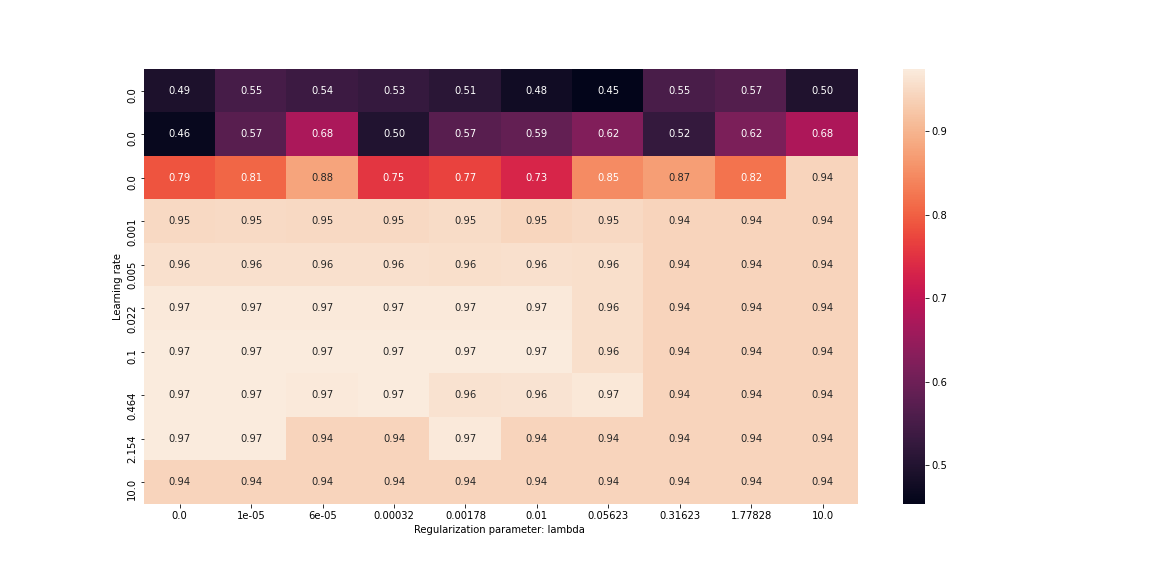
\includegraphics[trim=140 20 100 0, scale=0.3]{NNClass5}
	\caption{Accuracy score for third neural network model ploted over learning rate and regularization parameter.  }\label{figure}
\end{figure}
\begin{figure}[!htb]
	\centering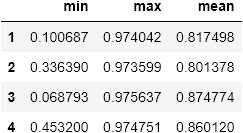
\includegraphics[trim=100 0 50 0, scale=0.6]{NNmodels}
	\caption{Max, min and mean accuracy score for the four neural network models over all parameters.  }\label{figure}
\end{figure}


\subsection{Support Vector Machine}
Training the SGDClassifier over the same values of learning rate and regularization parameter as the nerual networks. 
\begin{figure}[!htb]
	\centering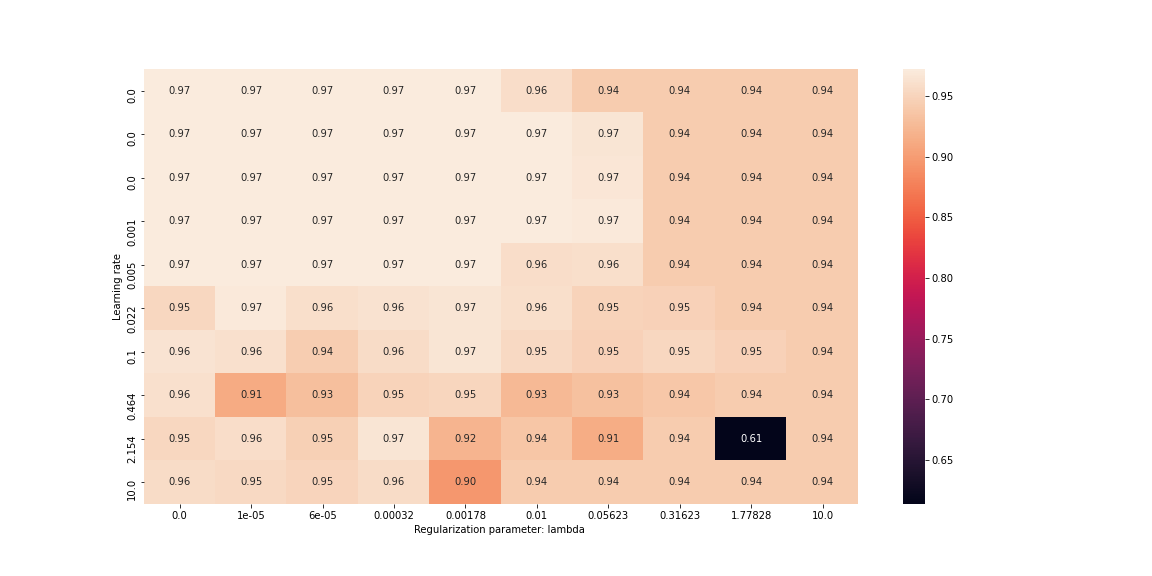
\includegraphics[trim=140 20 100 0, scale=0.3]{SGDClass}
	\caption{Accuracy score for SGDClassifier model ploted over learning rate and regularization parameter.}\label{figure}
\end{figure}
\begin{figure}[!htb]
	\centering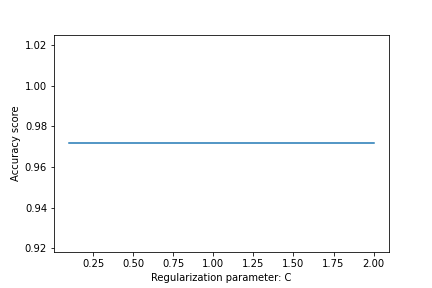
\includegraphics[trim=140 20 100 0, scale=0.3]{LinearSVC}
	\caption{Accuracy score for LinearSVC model over different values of C.}\label{figure}
\end{figure}



\section{Discussion}
The four different neural networks are performing fairly well at predicting the extended feature. All reaching a max accuracy score of atleast 97 \% with the best being model 3 with a score of 97,56 \%. 
All four models seems to be the most sensitive to learning rate. With the best performance between learning rates of 0,022 and 0,464. And with the lower range of learning rates performing significantly worse than the higher end. 
The regularization parameter seems to be less impactfull on the performance of the model, but there seems to be a slight bias to the lower end. 	
All four models seems to be able to reach a good performance over 97 \%. But model number 2 and 4 which are using the ELU activation function has higher minimum scores than the two others, not suffering as much from reduction in learning rate as the two other models. 
\newline
The SGDClassifier manage to reach the same level of performance as the neural networks with a max accuarcy score of 97.24 \%. But the SGDClassifier seems to have an over all better performance over the space of learning rates and regularization parameters. The worst score of the SGDClassifierer  is 61 \% which is higher than that of any of the neural networks. 

The LinearSVC model seem to be indifferent to the regularization parameter C, but nonetheless achievs a accuracy score corresponding to that of the other models of about 97 \%. The LinearSVC models takes a lot longer to train than the neural networks or the SGDClassifier which uses stochastic gradient descent.  

\section{Conclusion}

Both neural networks and support vector machines are able to classify an extended terror incident with quite high accuracy. There seemed to be little difference in the size of the neural network on the performance reached. But the networks that used the ELU activation function seemed to have a minimum performance that was quite higher than those that used the RELU function. 
The SGDClassifier managed to reach and equally good performance, but looked to perform better generally over all the parameters than the neural networks. The LinearSVC reached a good accuarcy score without any dependence on the regularization parameter C, but the model took a long time to train. I would conclude that the SGDClassifier performed overall better than the neural networks and was faster to train than the LinearSVC. 


\section*{References}  % the asterisk (*) after \section makes the section numbering go away
[1] https://www.kaggle.com/START-UMD/gtd \newline
[2] https://en.wikipedia.org/wiki/Support\_vector\_machine
\end{document}
